\documentclass[authoryear,12pt]{elsarticle}
\bibliographystyle{model2-names}
\usepackage{geometry}                % See geometry.pdf to learn the layout options. There are lots.
\geometry{letterpaper}                   % ... or a4paper or a5paper or ... 
%\geometry{landscape}                % Activate for for rotated page geometry
%\usepackage[parfill]{parskip}    % Activate to begin paragraphs with an empty line rather than an indent
\usepackage{graphicx}
\usepackage{amssymb}
\usepackage{epstopdf}
\usepackage{ulem}
\usepackage{url}
\usepackage{natbib}

\usepackage{wrapfig}
\usepackage{subfig}

\textwidth 6in
\textheight 9in

\graphicspath{{images/}}

\DeclareGraphicsRule{.tif}{png}{.png}{`convert #1 `dirname #1`/`basename #1 .tif`.png}

%\title{Flying \xout{On} Empty}
\title{Graphical Exploration of the Deep-Water Horizon Oil Spill}
\author{Lendie Follett, Ulrike Genschel, Heike Hofmann}
\date{\today}                                           % Activate to display a given date or no date

\begin{document}
\maketitle
%\tableofcontents
\begin{abstract}
\end{abstract}
\section{Introduction}
April 20th, 2010 marked the beginning of the largest and worst oil spill in the history of off-shore drilling.  Following an explosion in the Deep-Water Horizon drilling rig and failure of all emergency systems, crude oil began to gush into the ocean.  After an estimated 4.9 million barrels of oil spilled into the sea, the leak was finally stopped on July 15th of 2010 when the well head was capped.  The completion of the relief well took until September 19, 2010.  The immediate impact of the oil spill on people and wildlife alike was overwhelming and can still be felt.  The oil destroyed many habitats for birds, turtles, and other marine wildlife.  Waters had to be closed for fishing, affecting the livelihood of the people that depended on the fishing industry. Longterm effects are certain. It is of course impossible to do an analysis that can reflect the breadth and complexity of the effects of the oil spill.  However, based on the data provided by government sources we want to demonstrate the impact of the spill on wildlife, measured salinity - which has a major influence in determining oceanic flow, and environmental pollution through chemicals found in oil, in particular Polycyclic Aromatic Hydrocarbons (PAHs). 

\subsection{Data and Sources}
Data on dead and alive animal sightings came from several sources: US Fish and Wildlife (Southeast Region) provided the Cumulative Avian Observations (USFWS).
Data on Turtle \& Marine Mammal Observations were reported by NOAA (National Oceanic and Atmospheric Administration) and its offices NMS (National Marine Sanctuary) and OPR (Office of Protected Resources). 

Each of the files contains records of live and dead animal sightings, geographic location, exact species identification, if known, the date of the sighting, and, for the bird counts, a status variable regarding the oiling condition of the bird (Visibly Oiled, Not Visibly Oiled, Unknown). 


The EPA (US Environmental  Protection Agency) provided water and sediment chemistry data focused on petrochemical products, sampled near the coastline in the months since the oil spill. This file contained records of many chemicals and their geographic location, substance name, amount of substance, measuring unit, and date of measurement. 

Salinity data info*******

\subsection{Tools used}
*** what else did we make use of?

{\tt R} \citep{R2011}, {\tt ggplot2} \citep{ggplot2}, {\tt RgoogleMaps} \citep{RgoogleMaps}, link between {\tt ggplot2} and {\tt RgoogleMaps} provided by \citet{kahle2010} as part of his entry in the ggplot2 competition.

\subsection{Structure of this paper}
(structure)...
\begin{center}
\begin{tabular}{| l | p{11cm} | }
\hline
\multicolumn{2}{|c|}{{\bf Animals Data Set}} \\ \hline
Class & type of animal found: Birds, Sea Turtles, or Whales and Dolphins \\ \hline
Species & species of animal \\ \hline
Latitude & latitude in degrees  \\ \hline
Longitude & longitude in degrees\\ \hline
Alive & condition of animal: Alive or Dead. \\ \hline
Observation Date & date of observation 'mm-dd-yyyy'. \\ \hline
\multicolumn{2}{|c|}{{\bf Salinity Data Set}} \\ \hline
Date & date of observation. \\ \hline
Latitude & latitude in degrees \\ \hline
Longitude & longitude in degrees. \\ \hline
Depth & depth at which the measurement was taken in feet \\ \hline
Salinity &  measured amount of salinity. (mg/l) \\ \hline
Type &  type of measuring device used to take the measurement; Boat, Float or Glider \\ \hline
\multicolumn{2}{|c|}{{\bf Polycyclic Aromatic Hydrocarbons Data Set}} \\ \hline
Substance & PAH substance measured \\ \hline
Date & date of observation.\\ \hline
Latitude & latitude in degrees. \\ \hline
Longitude & longitude in degrees. \\ \hline
Result &  measured amount of the PAH substance. \\ \hline
Unit &  unit in which the PAH substance was taken; ug/L for water, ug/k for sediment. \\ \hline
Alkylation Multiplier* & given for each PAH substance to be used in calculations. \\ \hline
Acute Potency Divisor* &  given for each PAH substance to be used in calculations. \\ \hline
Chronic Potency Divisor* &  given for each PAH substance to be used in calculations. \\ \hline
Danger Level* &  health effects caused by the PAH substance; Carcinogen or other health effects. \\ \hline
\multicolumn{2}{|c|}{*these variables were taken from another source and put into the existing data set} \\ \hline
\end{tabular}
\end{center}

\section{Animal Sightings}
***  include the Google TM
*** The map for the sea turtles could be extended a bit and we could add state names (in white on the background)

\begin{figure}[htbp] %  figure placement: here, top, bottom, or page
   \centering
   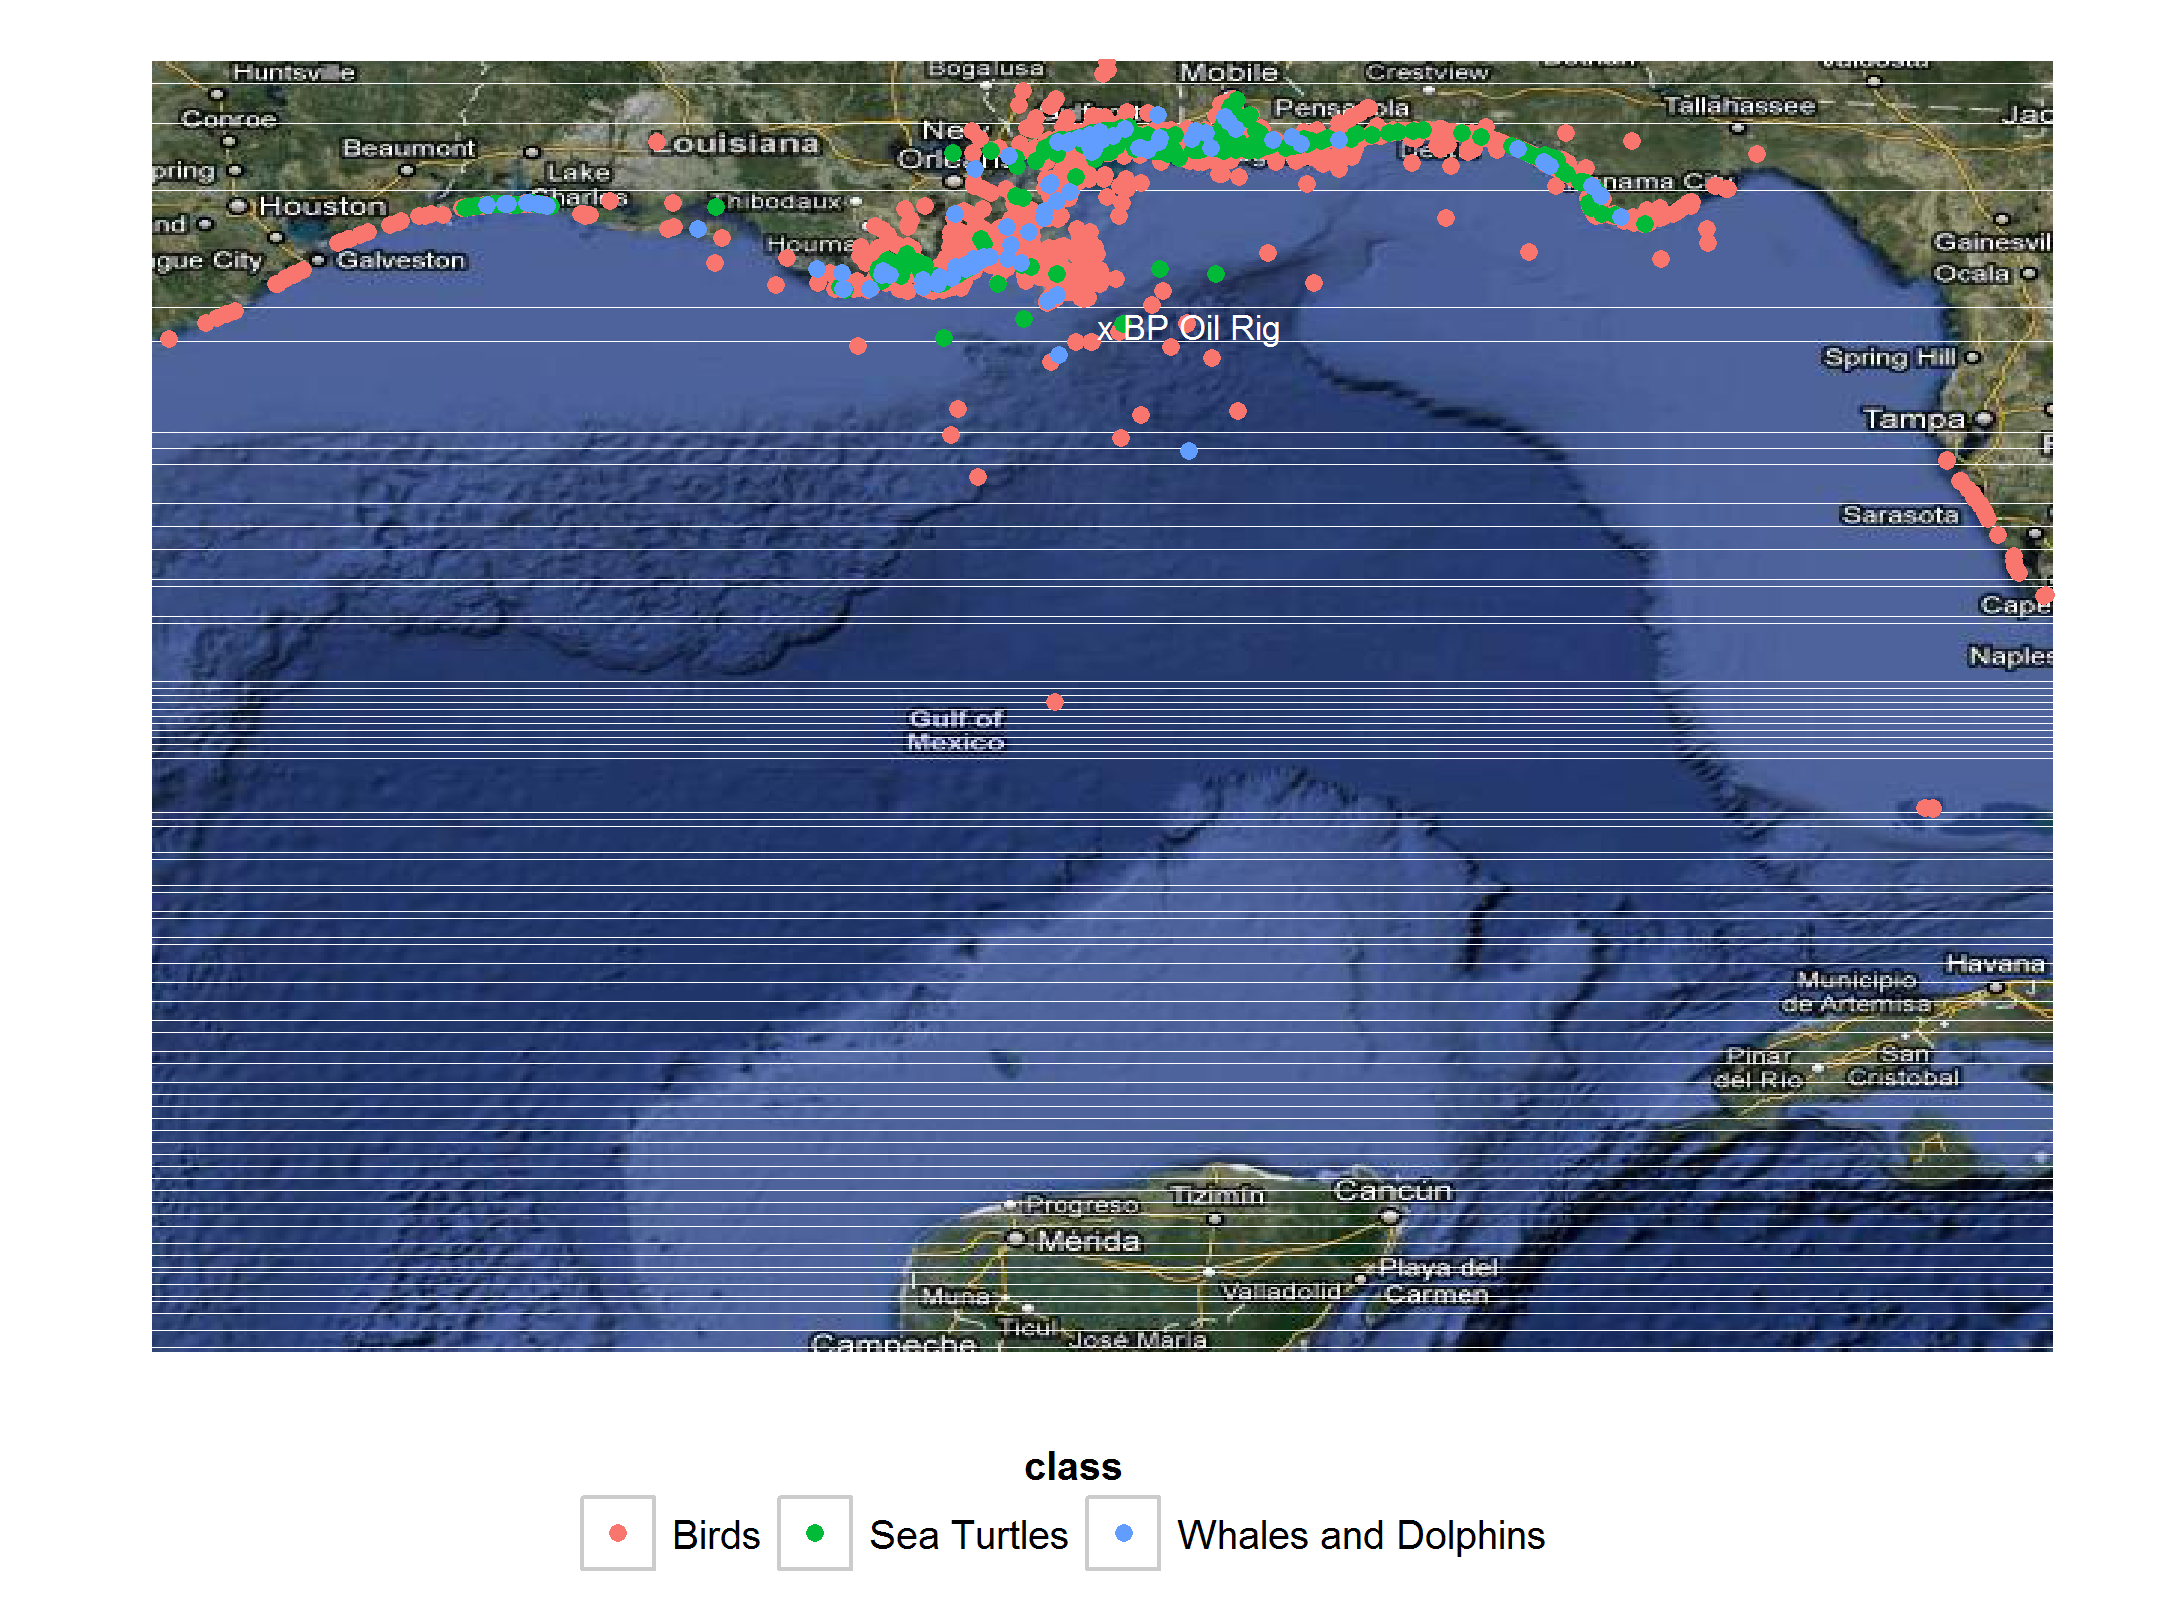
\includegraphics[width=4.5in]{animal_deaths.png} 
   \caption{Affected area: the graphic shows a satellite map of some of the area directly affected by the oil spill. The dots on top show locations of dead animal sightings. }
   \label{deaths}
\end{figure}
Figure \ref{deaths} shows a satellite map, overlaid by a dot plot indicating locations of animal sightings. Orange dots correspond to birds, yellow dots to sea turtles, and red dots to dolphins and whales.  Birds appeared to be most affected as a total of 5,552 dead birds were found and recorded during the data collection period.  A total of 546 sea turtles were found dead; all of the four identified sea turtle species are considered to be either threatened or endangered.  95 dolphins and 3 whales were found and recorded, all of which were dead. The highest concentration of dead animals was found along the shore of Louisiana, closest to the oil rig.  

\begin{figure}[htbp] %  figure placement: here, top, bottom, or page
   \centering
   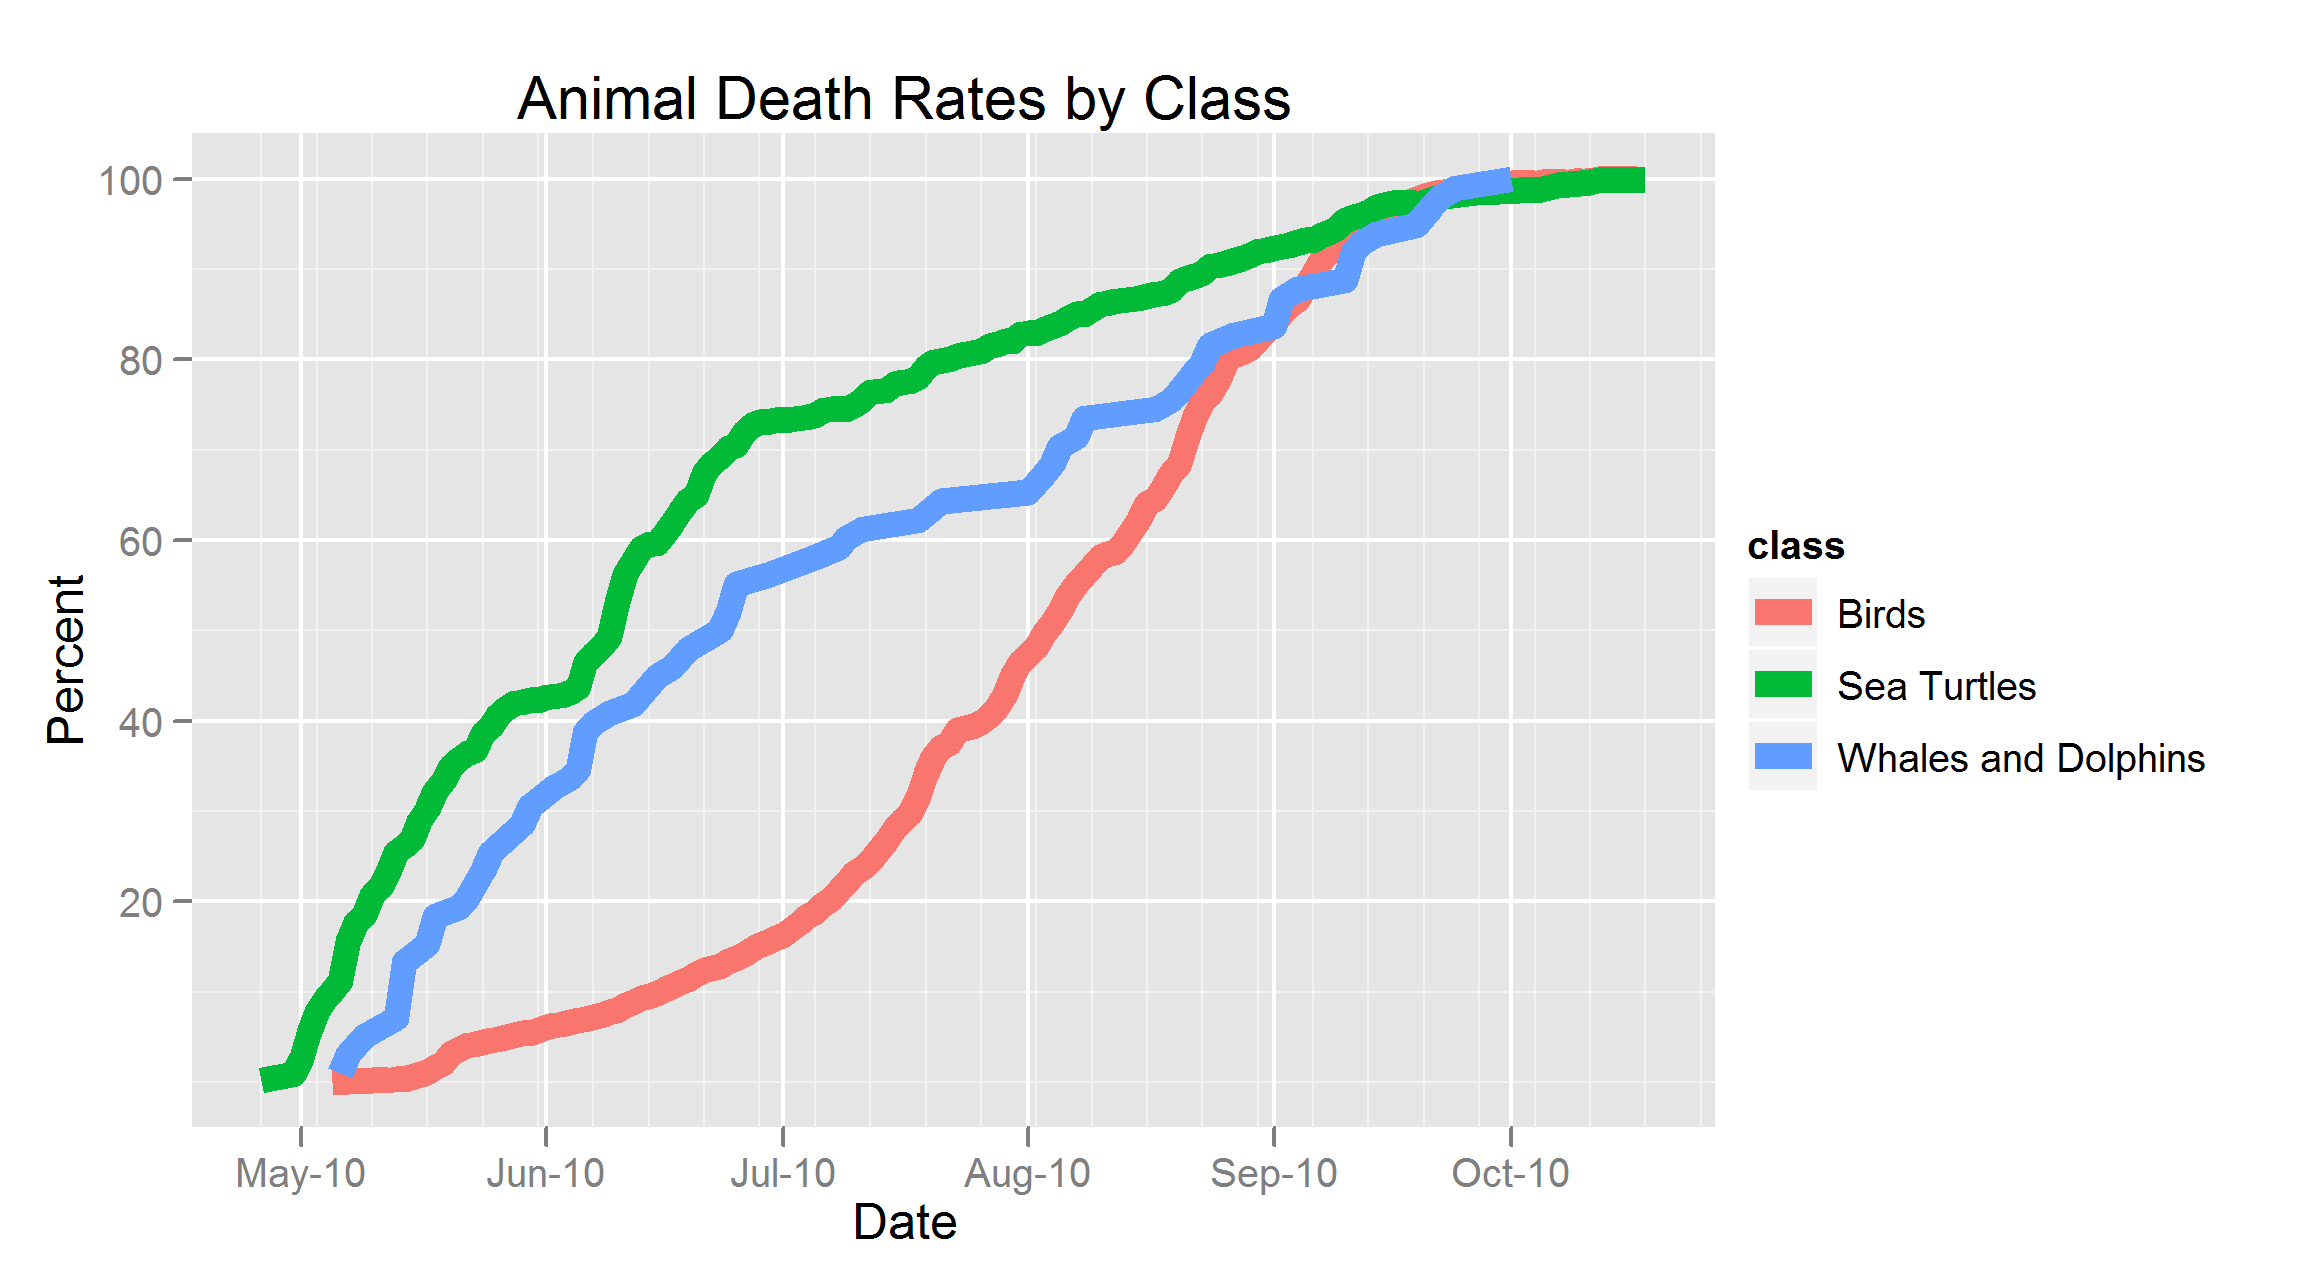
\includegraphics[width=1.9in]{death-rates.png} 
    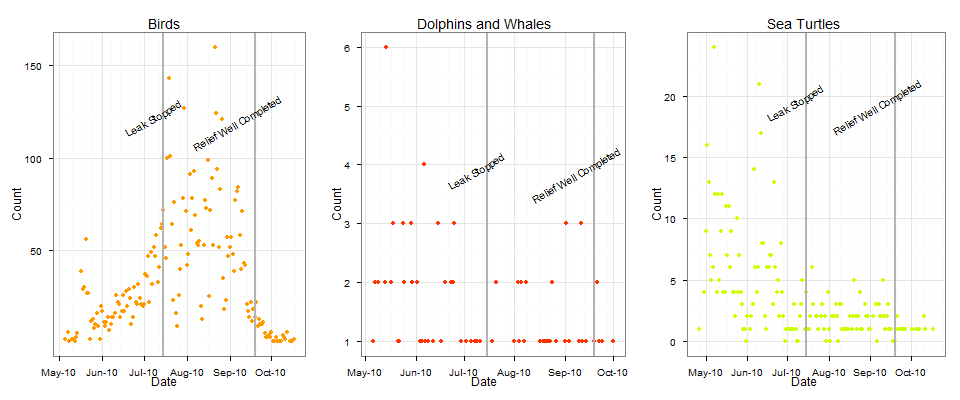
\includegraphics[width=3.9in]{daily-death-counts.png}
   \caption{The graphic on the left shows death rates of birds, dolphins, whales, and sea turtles from April to October 2010. The graphic on the right shows the daily number of dead animals found for each class of animal. The first vertical line at July 15th is when the leak was stopped and the well head was capped.  The second vertical line at September 19th is when the relief well was completed.}
   \label{death rates}
\end{figure}

\begin{table}[ht]
\caption{Number of Dead Animals: April 26, 2010 to October 18, 2010}
\centering
\begin{tabular}{c c c c}
\hline\hline
Birds & Dolphins and Whales & Sea Turtles & Total \\ [0.5ex]
% inserts table
%heading
\hline
% inserts single horizontal line
5,552 & 98 & 546 & 6196\\ [1ex]
% [1ex] adds vertical space
\hline
%inserts single line
\end{tabular}
\label{table:table1}
% is used to refer this table in the text
\end{table}

Birds, sea turtles, and dolphins and whales had unique death patterns during the data collection period as Figure \ref{death rates}  illustrates. In the left figure, the to-date death toll was divided by the total death toll for each class of animal. The birds had a relatively low death rate from May to July and then the rate began to increase. Sea turtles and dolphins and whales, on the other hand, had the highest death rates from May to July and from there it began to flatten out. These patterns can also be seen in the figure on the right, which shows daily death counts for each class of animal. For sea turtles, dolphins, and whales, the highest death counts per day occurred mainly in the earlier weeks and then decreased over time.  The majority of dead bird findings occurred later in time and their death counts per day began to climb rapidly around July. From July to September, the birds experienced a wide range of death counts per day and then began to decrease at the end of September. By October 18th, 6,196 birds, sea turtles, whales, and dolphins had been identified as dead. 

\begin{figure}[htbp] %  figure placement: here, top, bottom, or page
   \centering
   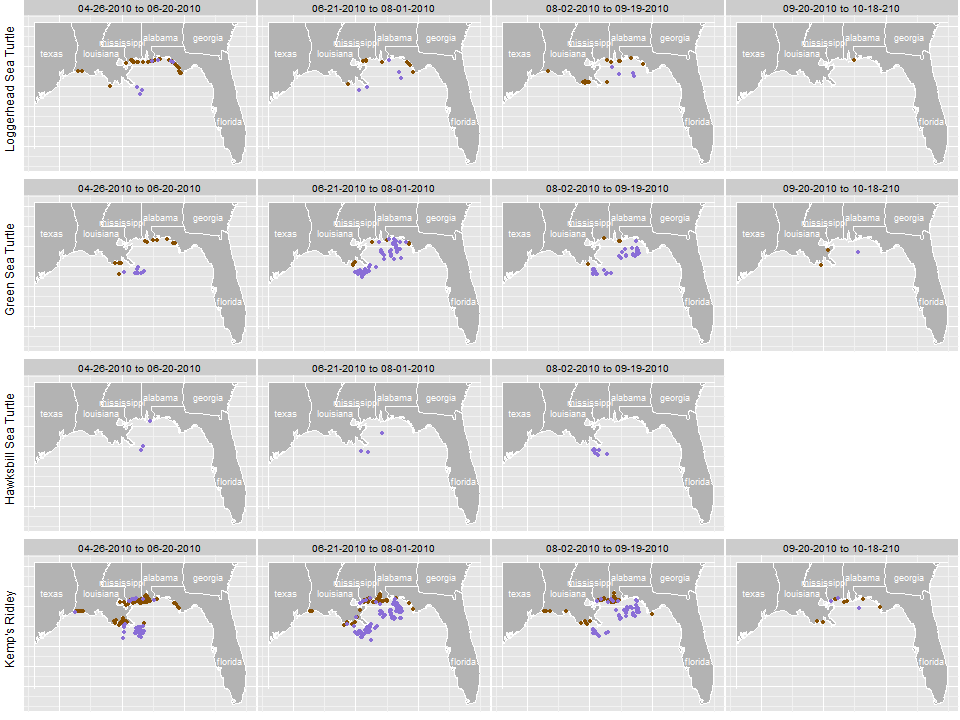
\includegraphics[width=6in]{turtles.png} 
   \caption{Four species of endangered or critically endangered sea turtles found in the Gulf of Mexico from April 26th to October 18th 2010.  Yellow dots indicate turtles found living and orange dots indicate those found dead.}
   \label{turtles}
\end{figure}

Four species of sea turtles were found and identified during the data collection period, all of which are considered to be either threatened or endangered. These species are: Kemp's ridley, Hawksbill Sea Turtle, Green Sea Turtle, and Loggerhead Sea Turtle. Figure \ref{turtles} shows when and where these turtles were found and whether they were living or dead. Most dead turtles, of all species, were found along the shoreline. Most turtles that were found alive were found off the coast. There were two main areas on the coasts of Louisiana and Florida in which the bulk of live sea turtles were found.  This is most evident among the Green Sea Turtle and Kemp's ridley.Very few turtles were found after September. The species with the greatest number of casualties found was Kemp's ridley, an endangered species which lives primarily in the Gulf of Mexico.  It is more common for Kemp's ridley sea turtles to be present in the northern part of the Gulf of Mexico during June, July, and August. Female Kemp's ridleys, like other sea turtles, nest between May and July and lay their eggs on various beaches of the Gulf of Mexico  \citet{turtles}. From this information, we can understand that there were more turtles in the area during the months after the oil spill occured, and thus more sea turtles to be found.  After August, however, it would be natural for these turtles to begin to leave the area and head south.

\section{Chemicals}


Various chemicals were sampled in the Gulf of Mexico during the months following the oil spill. This analysis focuses on Polycyclic Aromatic Hydrocarbons firstly because of their direct relationship with oil and secondly because of their toxicity to wildlife. Polycyclic Aromatic Hydrocarbons, or PAHs, are semi-volatile organic substances which come mainly from oil and the burning of oil. However, they can also come exhaust and from the burning of gas, coal, garbage and other organic substances \citep{pah}.   Many of these substances are considered carcinogenic, mutagenic, and teratogenic and all are considered harmful to the health of living organisms. New information on each PAH substance was found from the EPA website  \citep{pah} and put into the data set for this analysis. In order to do a proper analysis on the existence of these chemicals after the spill and how they may have effected life in the Gulf of Mexico it was necessary to put the measurements into an interpretable form. We followed the approach by \citet{pah-benchmark}: measurements of the PAHs at unique locations will be looked at in terms of their acute and chronic potency. An area is considered at a chronic level when the amount of harmful substances is thought to bring harmful effects over a long period of time. An area is considered at an acute level when the amount of harmful substances rapidly induces a negative effect in an organism. The following describes the process in which we could analyze these PAHs in terms of their acute and chronic levels. 
\begin{center} \textbf{Sediment} \end{center}

Each PAH substance has a unique acute and chronic potency divisor which is used to find the acute and chronic potency ratio, respectively. The potency divisors, which are used in the calculations, can be thought of as the amount of the substance that can be considered dangerous by itself. So, each measured amount of a substance is divided by the chronic and acute potency divisors so that, at each location, we have a ratio of the danger. For surface water and sediment samples alike, these ratios are additive and each substances' contribution must be summed up for each unique location in order to determine the complete effect. The following formulas show how we attained the chronic and acute benchmark values for water and sediment. After all of this was done, several areas along the beaches of the Gulf of Mexico were found to be at a chronic or acute level. 

$Chronic Benchmark Value = \sum \frac{Alkylation Multiplier \times Measured Amount of Substance (ug/L)}{Chronic Potency Divisor}$

$Acute Benchmark Value = \sum \frac{Alkylation Multiplier \times Measured Amount of Substance (ug/L)}{Acute Potency Divisor}$
\begin{center} \textbf{Sediment} \end{center}

$Chronic Bencmark Value = \sum \frac{(\frac{Measured Amount of Substance (ug/kg)}{Organic Carbon}) \times Alkylation Multiplier}{Chronic Potency Divisor}$

$Acute Benchmark Value = \sum \frac{(\frac{Measured Amount of Substance (ug/kg)}{Organic Carbon}) \times Alkylation Multiplier}{Acute Potency Divisor}$

For substances measured in sediment, the amount of organic carbon for that area must  be used to find the acute and chronic potency ratios. Taking the organic carbon into consideration is important for sediment samples because, when it is present in the sediment, the PAHs bind to it, thus making the PAHs less toxic. Organic carbon, like any other substance, was measured at each location. These concentrations of organic carbon at each unique location were put into a separate data set. Then, the organic carbon data set and the PAH sediment data set could be horizontally merged by unique combinations of Latitude and Longitude. This is done so that each measured concentration of a PAH substance has an accurate corresponding organic carbon measurement. 


\begin{figure}[htbp] %  figure placement: here, top, bottom, or page
   \centering
   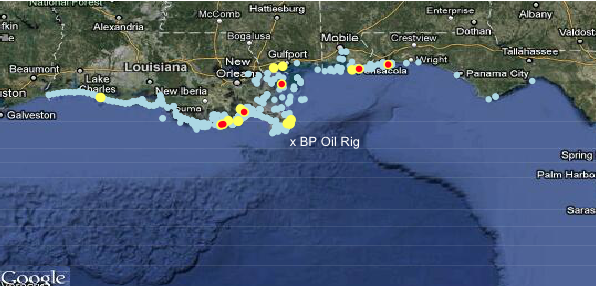
\includegraphics[width=5in]{chron-acute-map.png} 
   \caption{Map showing PAH measurements. Yellow dots represent those considered at a chronic level, red dots represent those considered at an acute level.  Light blue dots indicate all samples.  Most dangerous area seems to be around the outermost shore of Louisiana as there are many points which had PAH levels at or above chronic or acute benchmarks.}
   \label{pah-map}
\end{figure}


Figure \ref{pah-map} shows areas which meet or exceed the chronic and acute benchmarks.  The yellow dots represent areas which meet or exceed the chronic benchmark and the red dots represent areas which meet or exceed the acute benchmark.  The light blue dots indicate all areas which were tested.  For this graphic, average values of each substance for each unique location were used.  This way, there is exactly one measurement of each substance at each location.  There were several areas which had dangerous levels of these PAH substances.  Particularly along the outer coast of Louisiana, many of the observed PAH values exceeded the benchmarks.  This is the area which may have received the most direct contact with the oil.  

\begin{figure}[htbp] %  figure placement: here, top, bottom, or page
   \centering
   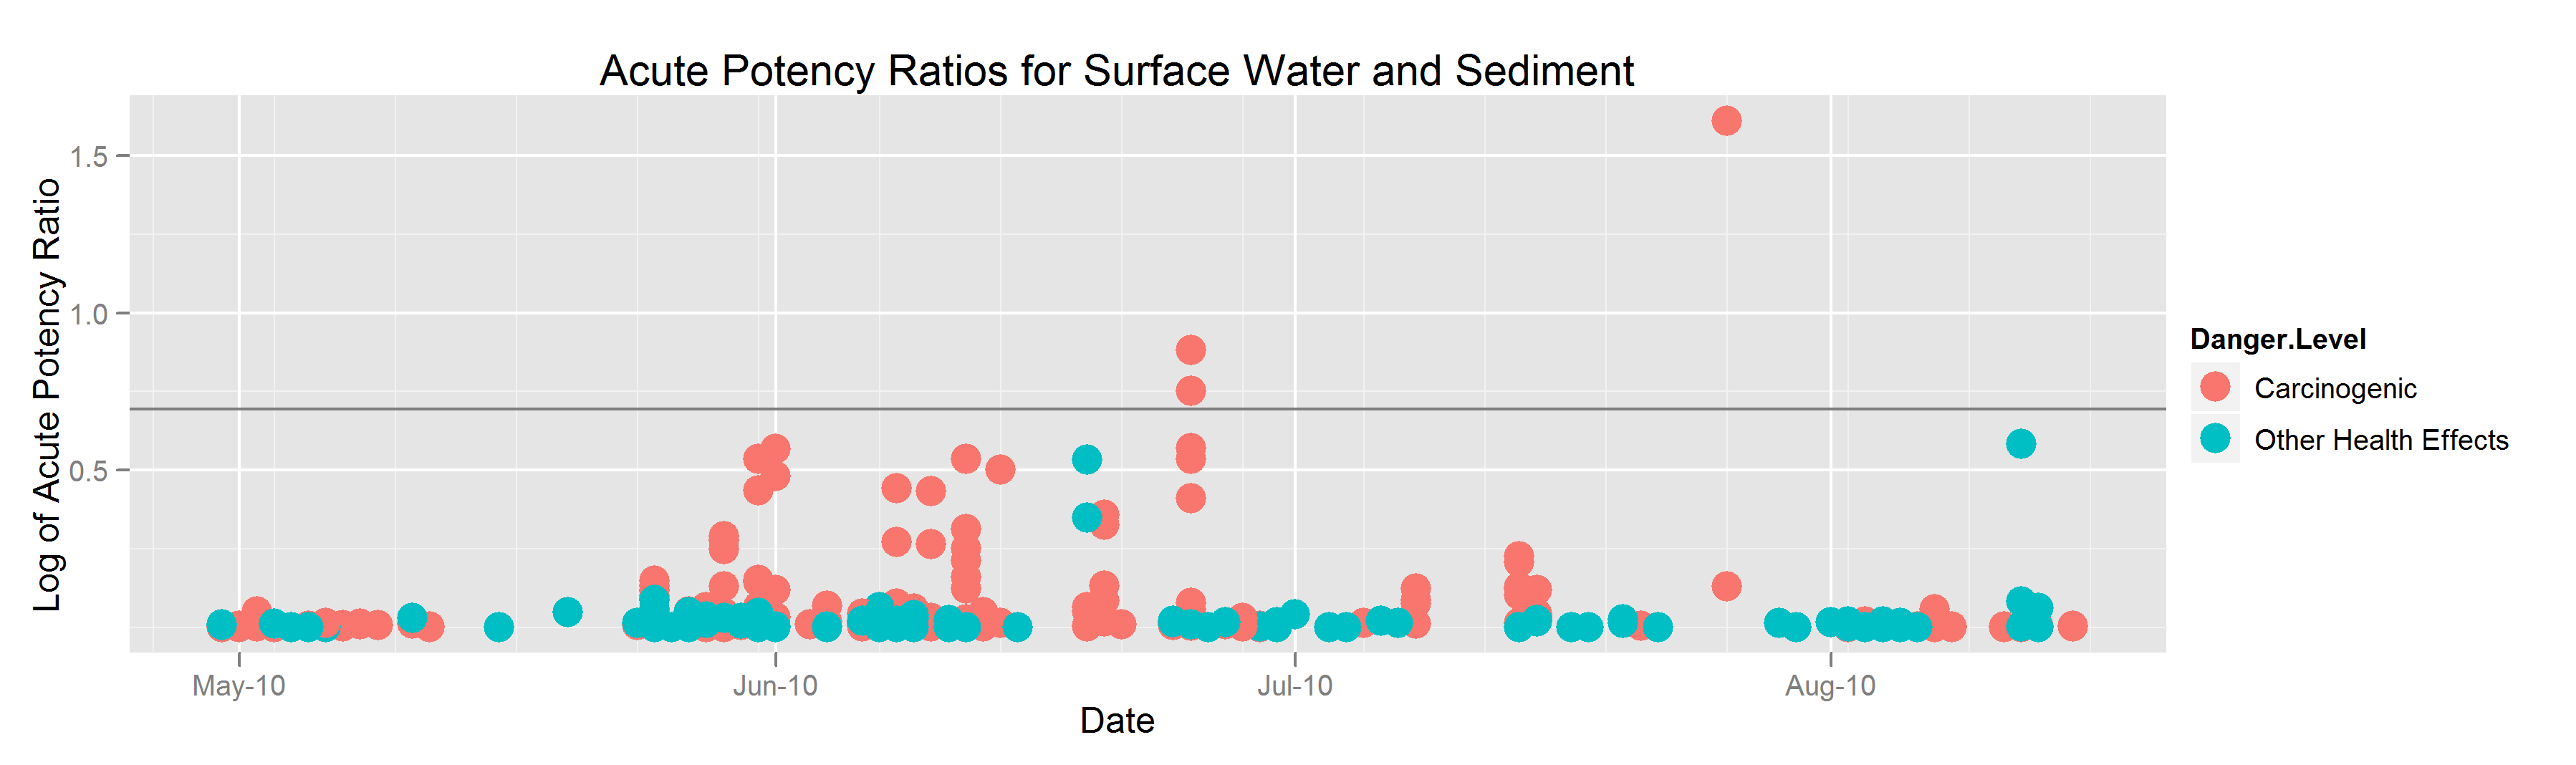
\includegraphics[width=5in]{acute-timeline3.png} 
   \caption{Timeline of logarithm of acute potency ratios.  Points are colored by the substance's effect on health. There is a period of time between June and July in which the acute value is heightened.  Points which alone exceed the acute benchmark are labeled with the name of the substance.}
   \label{pah-timeline}
\end{figure}


Figure \ref {pah-timeline} shows the log of the acute potency ratios not equal to 0 for measurements taken from May 2010 to August 2010. The log was taken so that we could more easily see the variation, as many of the samples were near 0. Some measurements of PAH substances exceeded the acute potency ratio alone, meaning that, even if there were no other PAH substances in the area, that one substance was enough to be acutely dangerous. These three acutely dangerous measurements are labeled on the timeline as C1-Chrysenes, C2-Chrysenes, and Chrysene. The Chrysene family is considered a carcinogenic substance. There seems to be a period of time between June and July in which the measurements of these PAH substance had higher values than during the rest of the time.

\section{Salinity}
Boats, floats, and gliders recorded salinity, temperature, and depth measurements at various locations in the Gulf of Mexico. The floats tended to stay in the deeper water while the boats and the gliders were free to go all around the gulf.  You can see the patterns of these three measuring methods in Figure \ref {Boats, Floats and Gliders}. Each measuring device would take measurements at the surface and then take measurements at various depths at each location.  

\begin{figure}[htbp] %  figure placement: here, top, bottom, or page
   \centering
   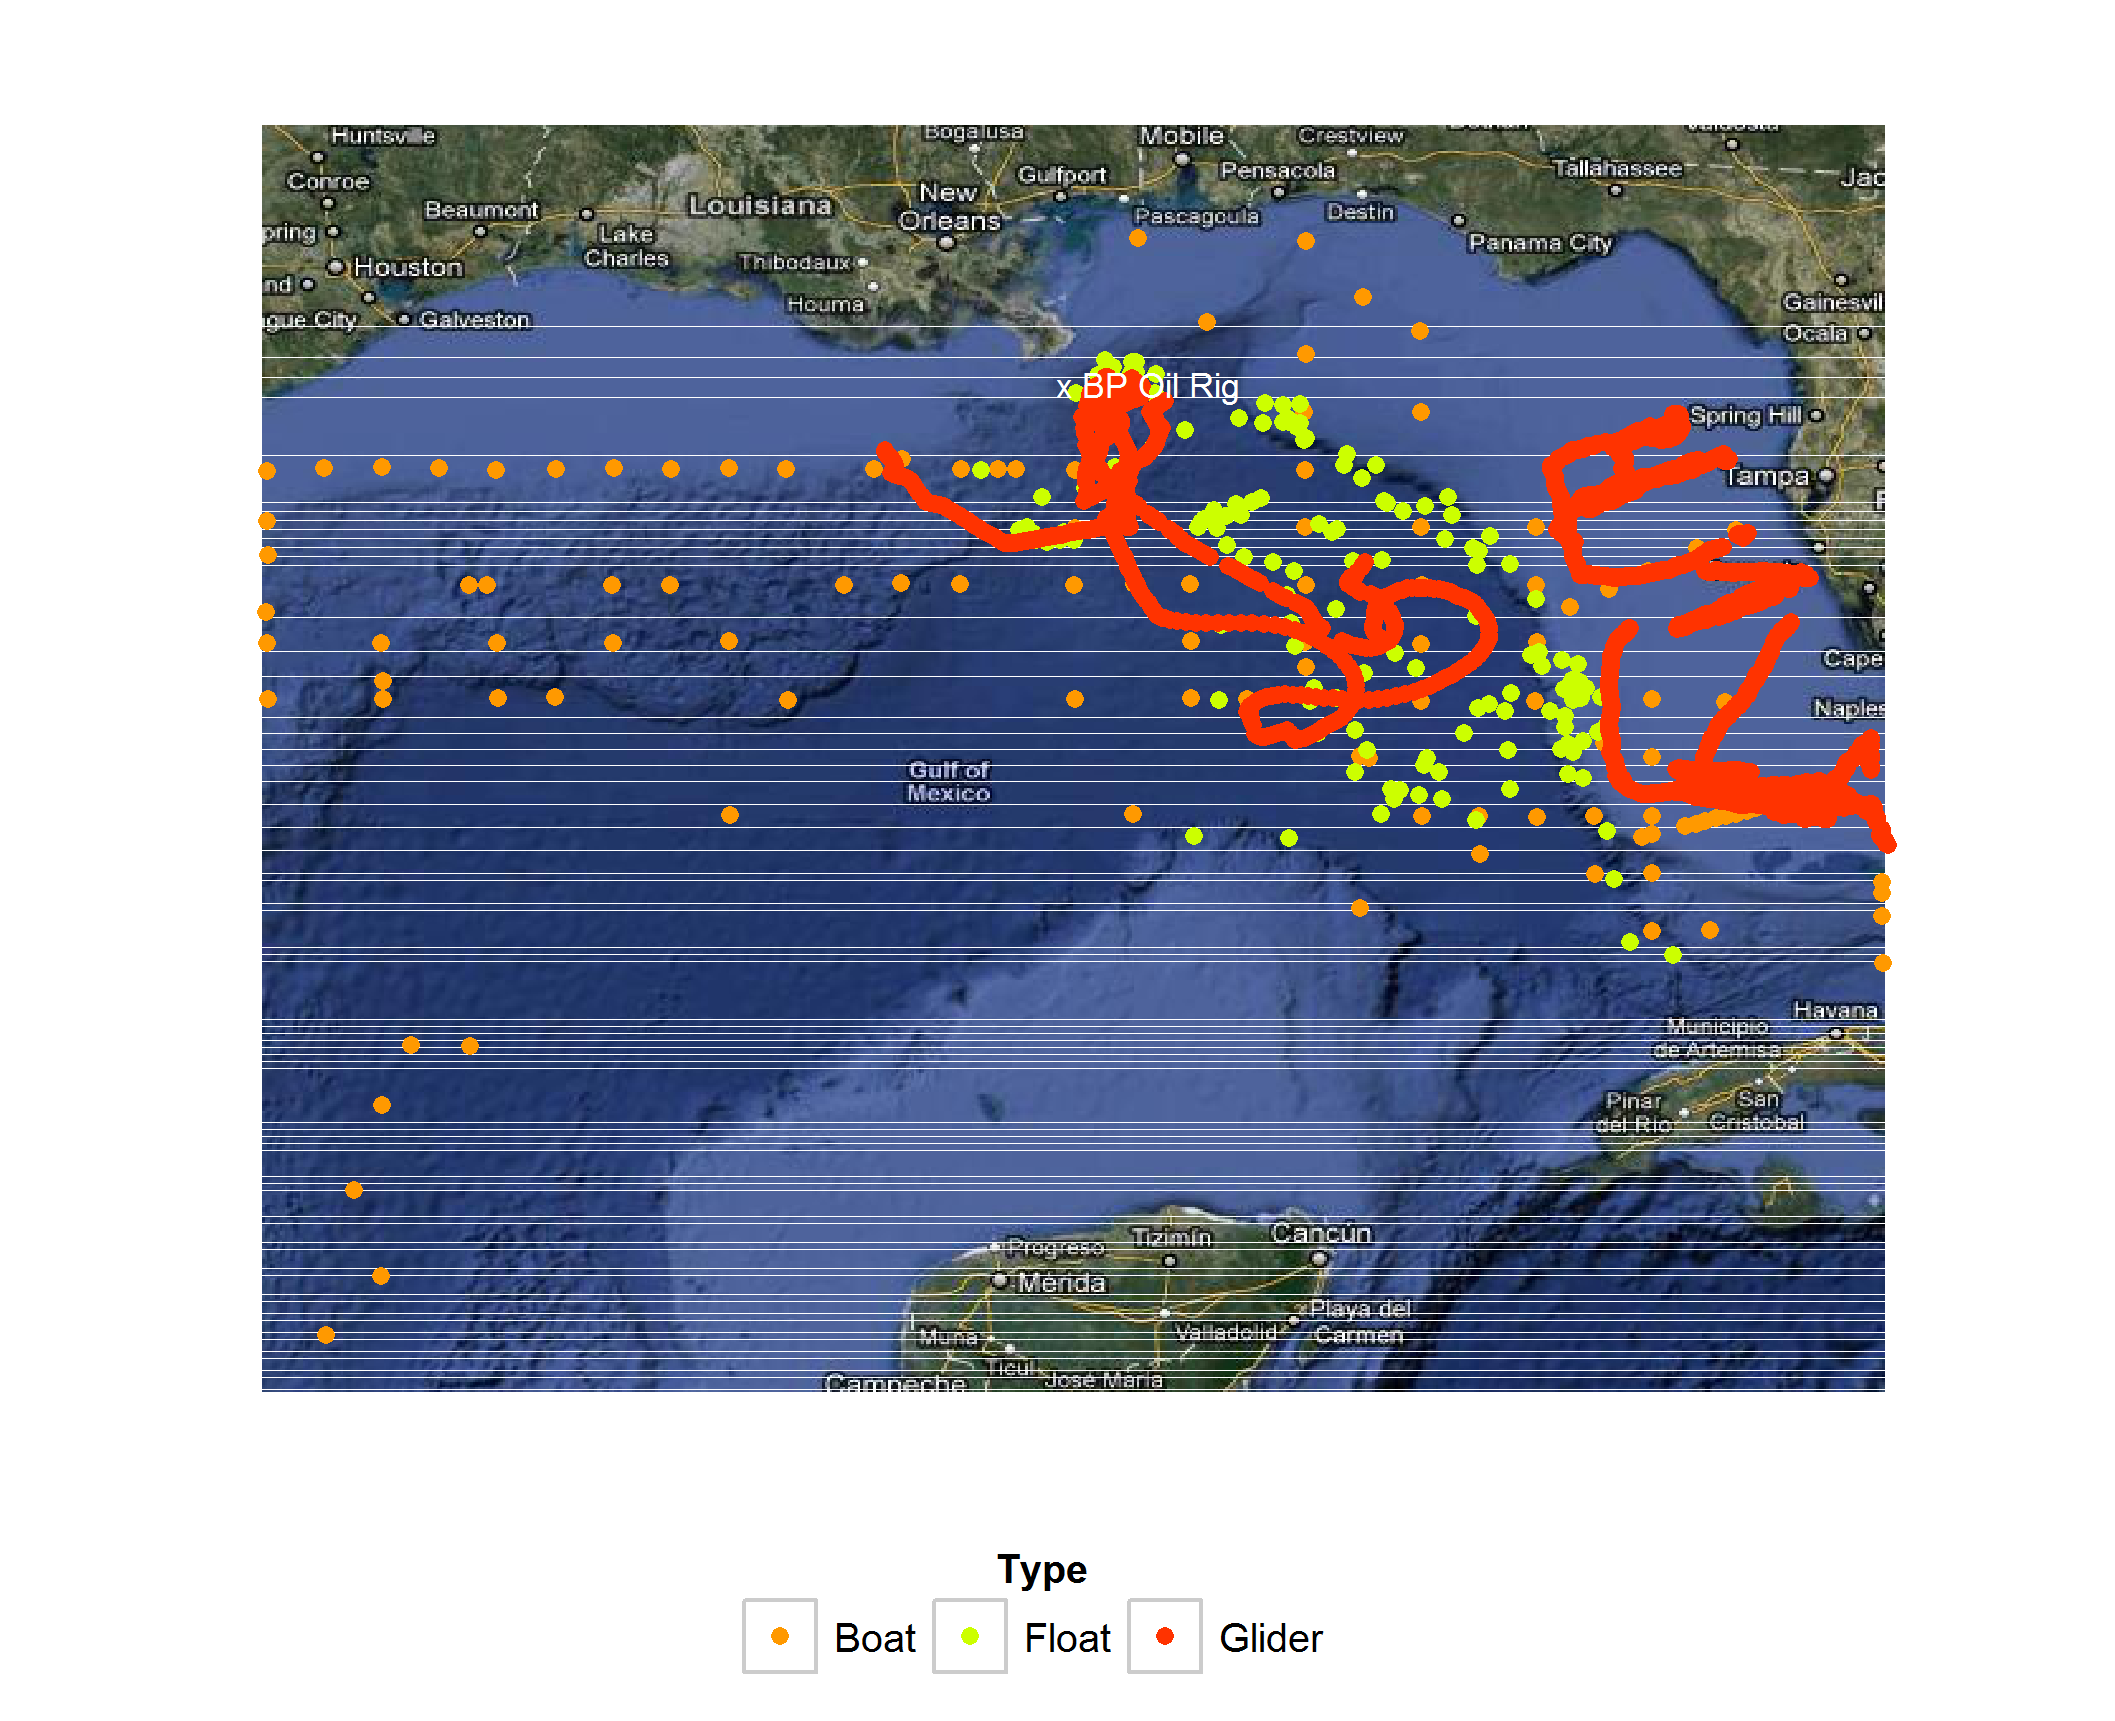
\includegraphics[width=5in]{boats-floats-gliders.png} 
   \caption{Paths of Boats, Floats, and Gliders. }
   \label{Boats, Floats and Gliders}
\end{figure}
In Figure \ref {salinity-timeline} you can see all salinity measurements over the data collection period. In both the left and right graphic, the points are color coordinated by time. The right graphic shows only points where salinity levels are below 34 mg/l. The vast majority of the salinity measurements stayed within set boundaries. Other points varied from the rest and seemed to be unusually low. In the right graphic of Figure \ref {salinity-timeline} you can see when and where these unusual values occurred. The highest concentration of these points is found near the rig during June and July.
\begin{figure}[htbp] %  figure placement: here, top, bottom, or page
   \centering
   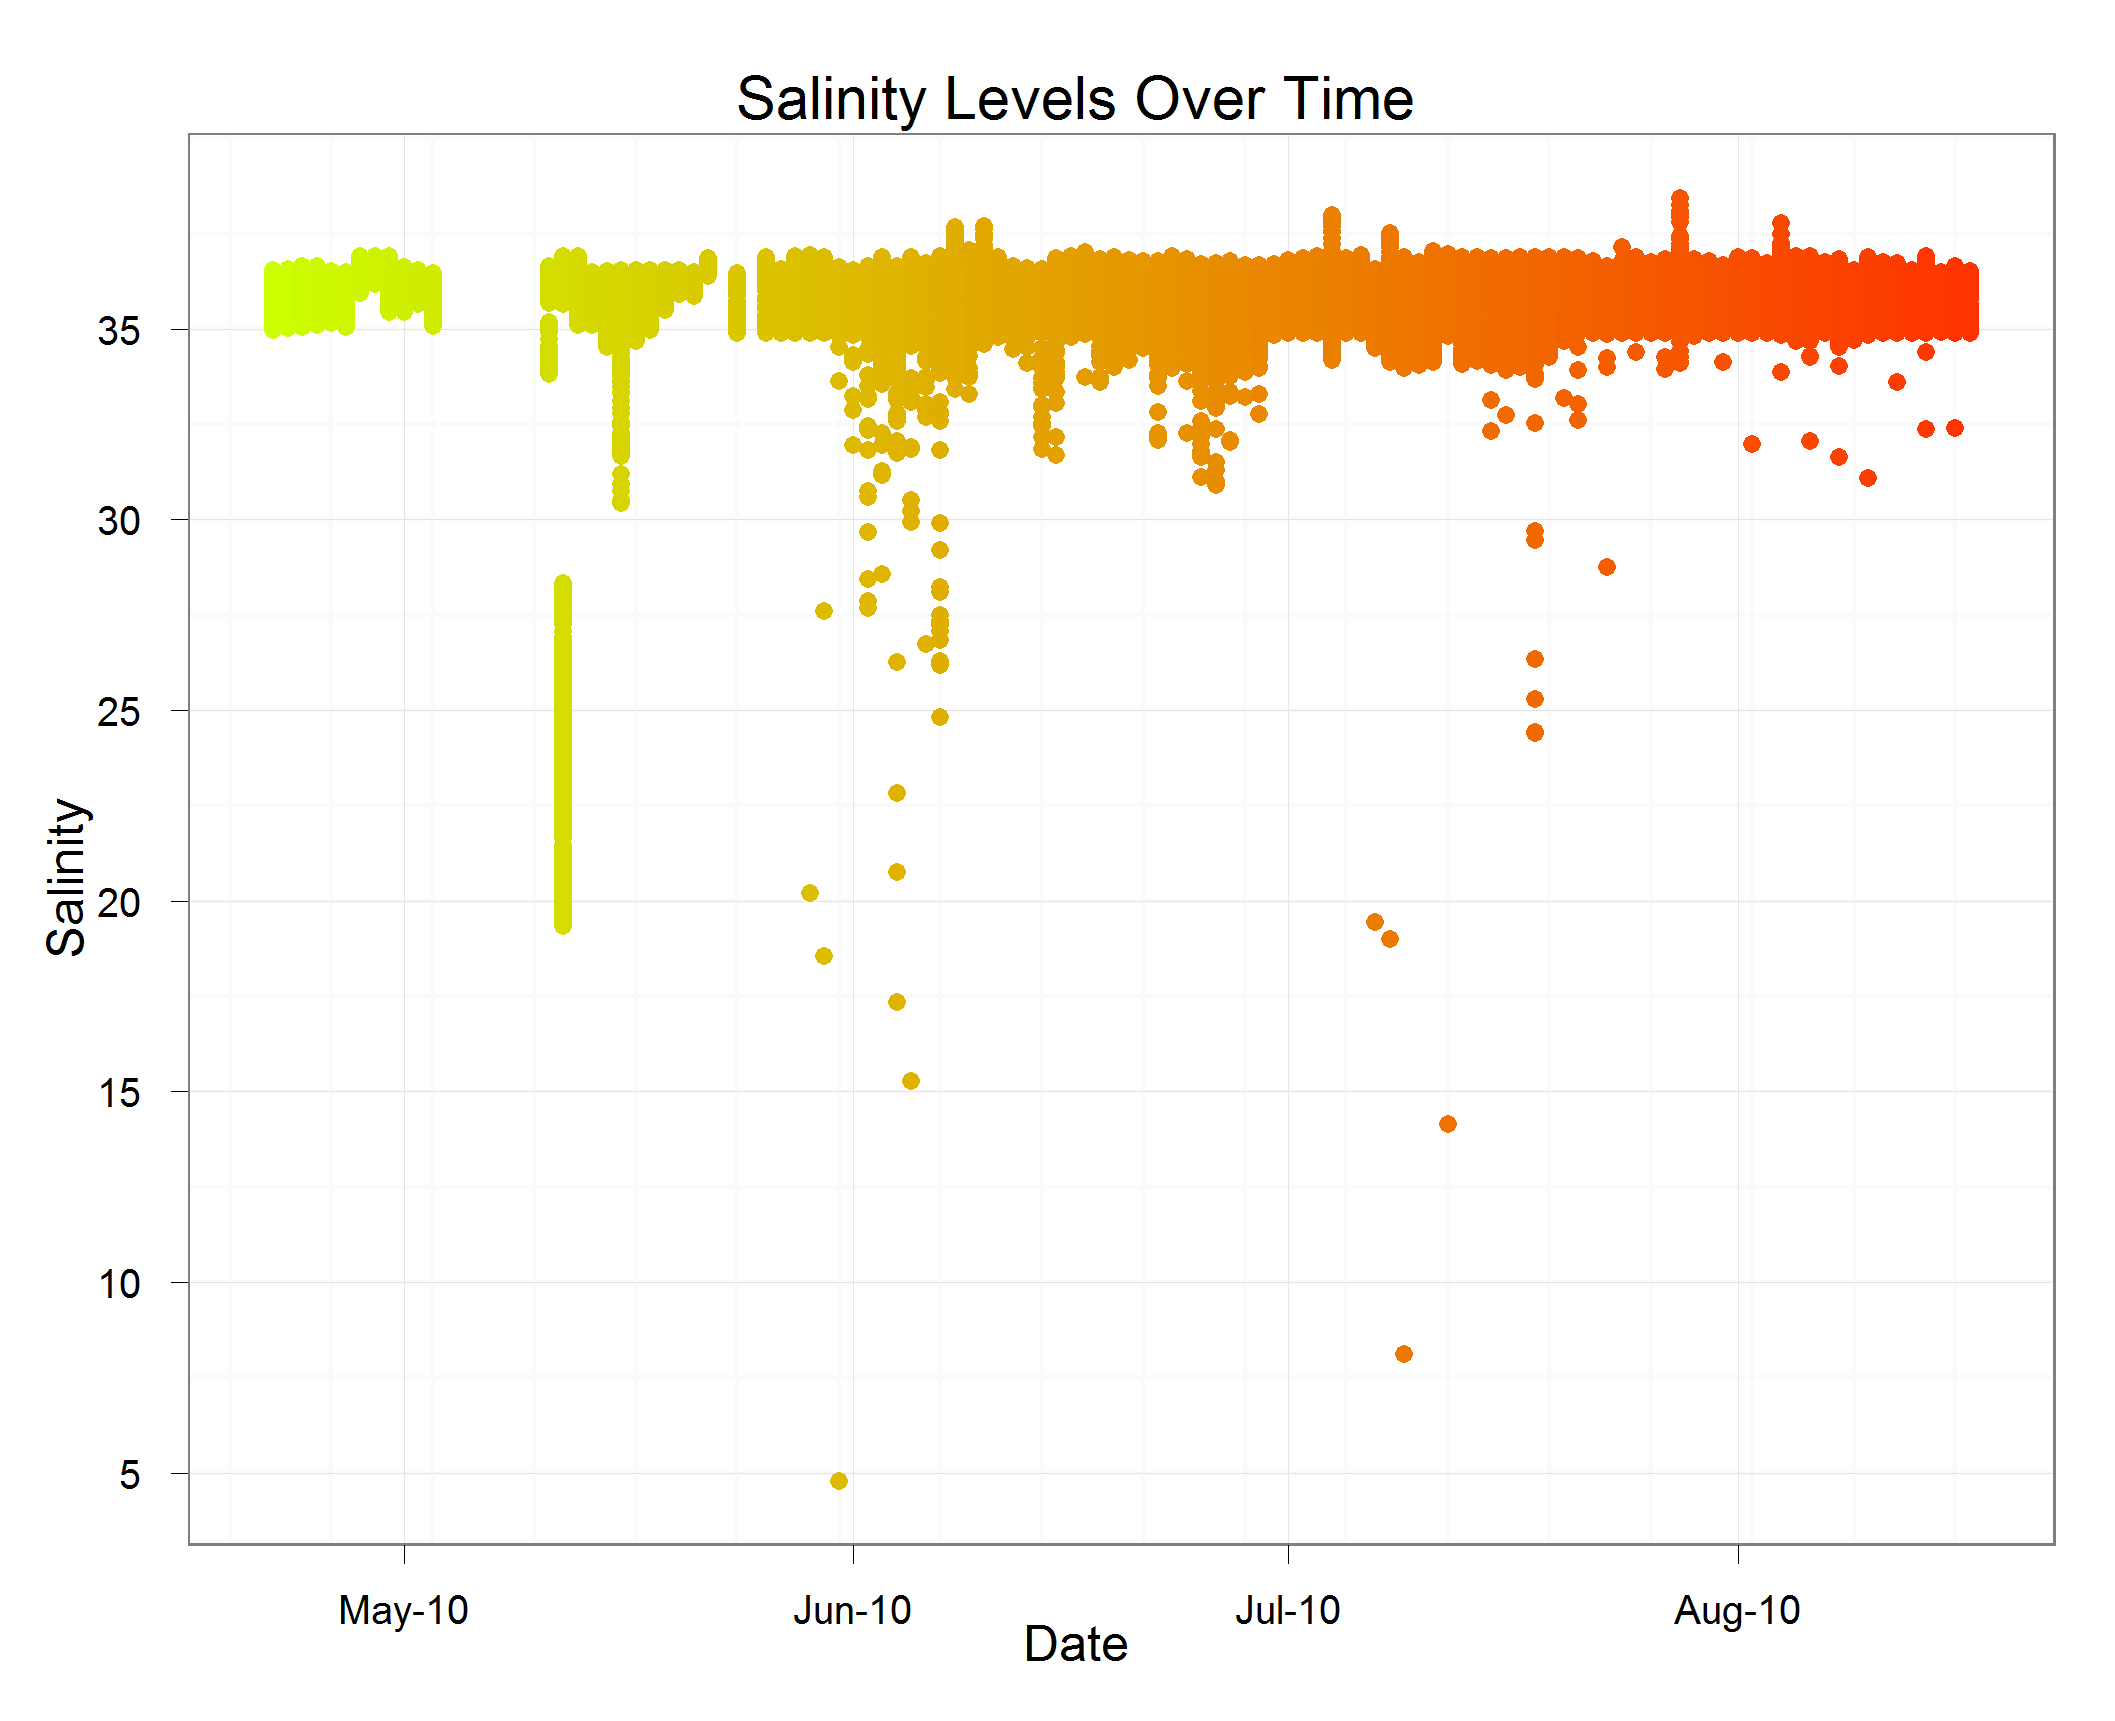
\includegraphics[width=2.8in]{salinity-time.png} 
   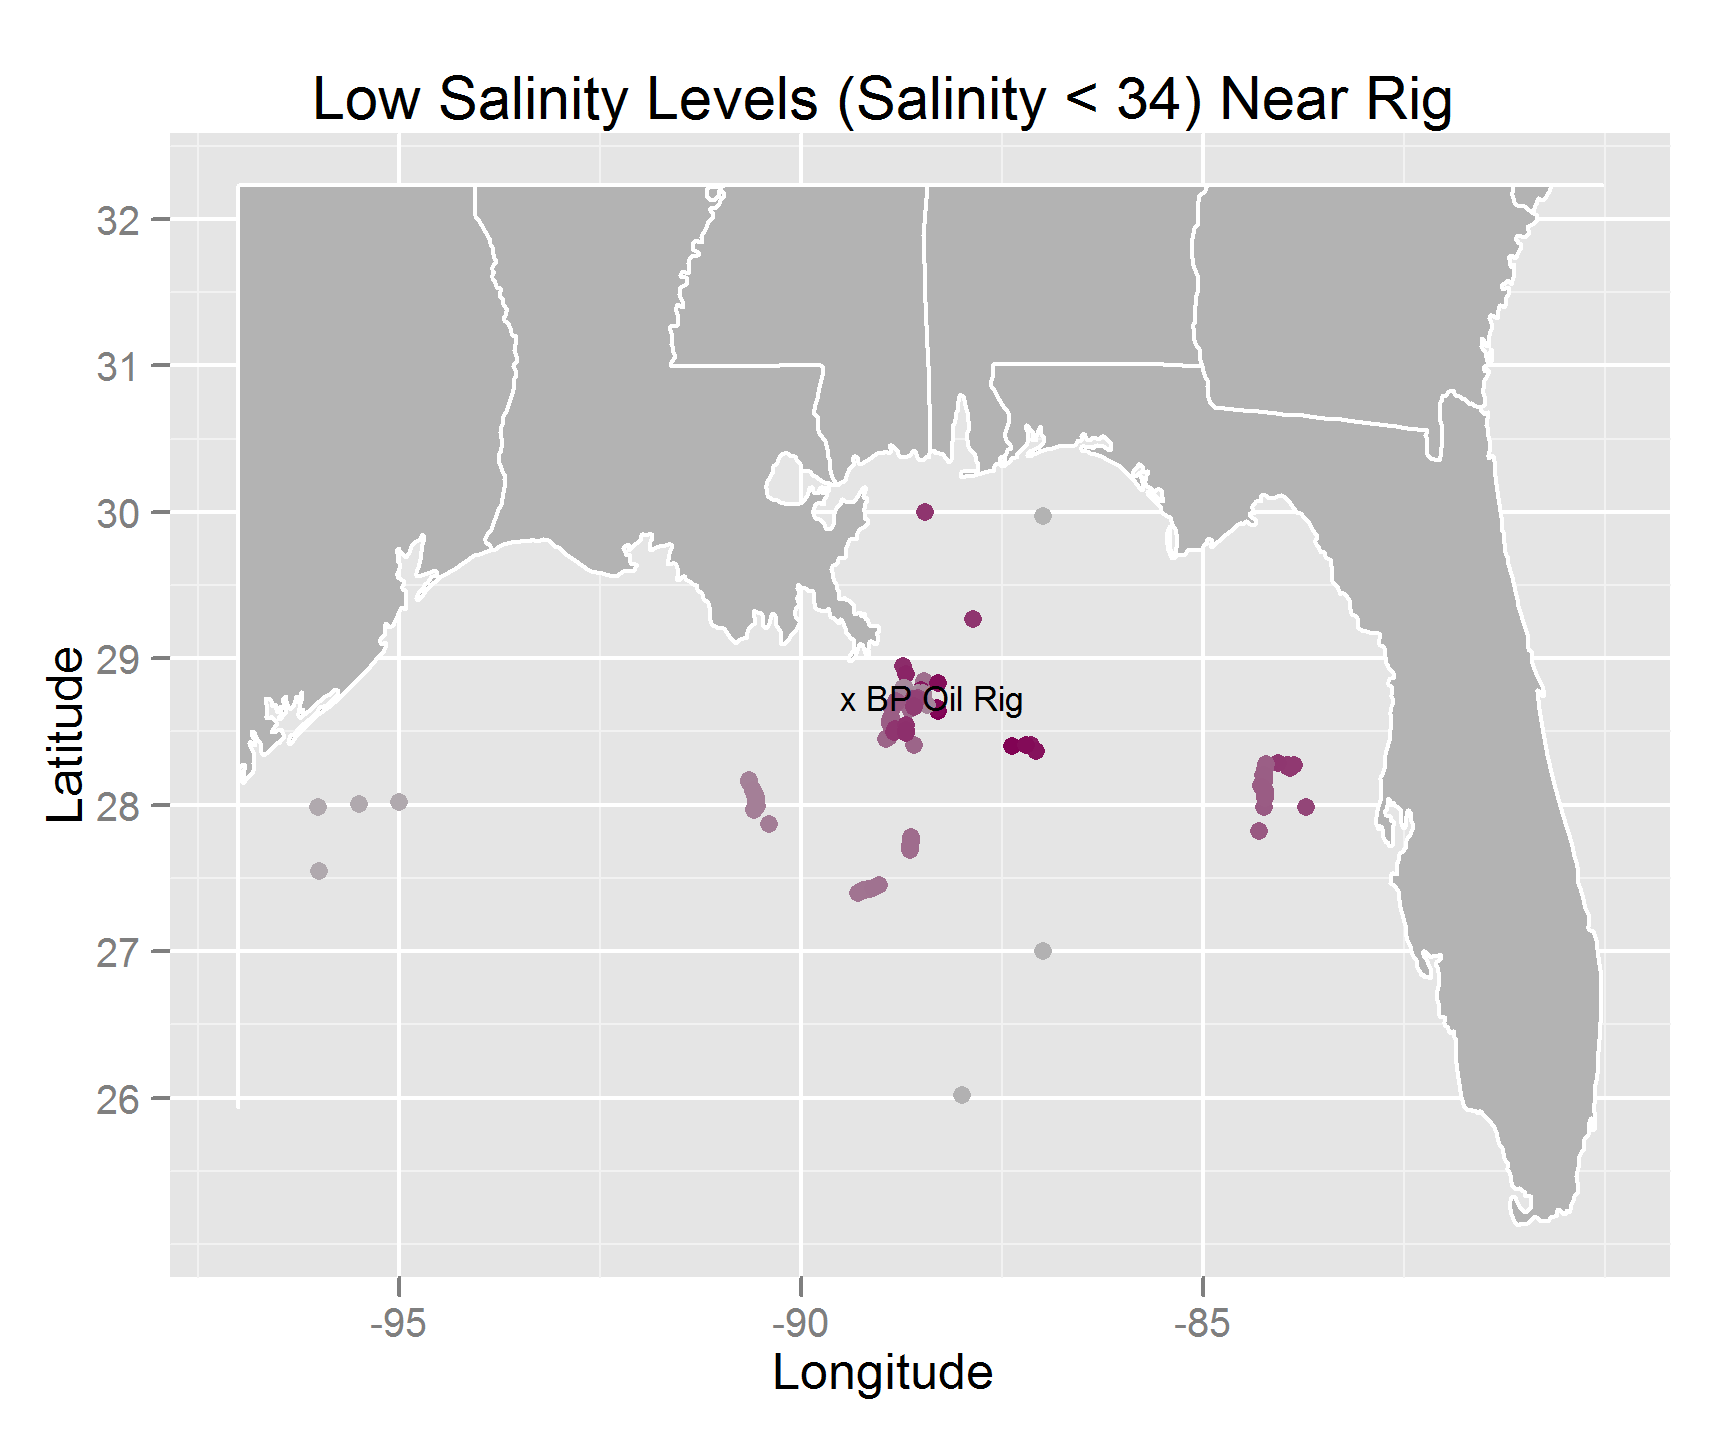
\includegraphics[width=2.8in]{salinity-map.png} 
   \caption{Salinity measurements: over time (left) and by location (right)> Salinity measurements only rarely fall below 34 mg/l. In the months after the start of the oil spill salinity frequently drops below 34 mg/l. For later weeks this happens in particular in locations close to the oil rig.}
   \label{salinity-timeline}
\end{figure}

\begin{figure}[htbp] %  figure placement: here, top, bottom, or page
   \centering
   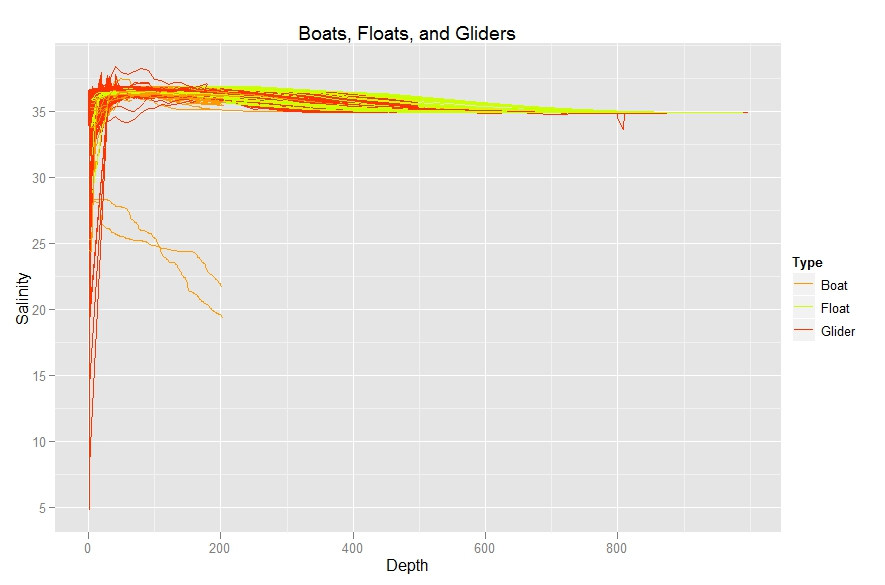
\includegraphics[width=4in]{salinity-depth.jpeg} 
   \caption{Relationship between depth and salinity grouped by each unique latitude and longitude combination. Depth and salinity almost always maintain a fixed relationship, as seen in most of the observations. However, some areas, mainly those at the surface of the water, experienced unusually low values of salinity. Two areas, which were measured by a boat, had a depth-salinity relationship very unlike the rest.}
   \label{Depth-Salinity}
\end{figure}
Depth and salinity form a close relationship as you can see in Figure \ref {Depth-Salinity}. Normally, salinity levels would stay between 38 and 34 mg/l. This trend was violated for many measurements taken near the surface but then resumed normal measurements at greater depths. There were also two measurements taken by a boat which do not follow the normal relationship. The surface water measurement was far below normal observations and from there salinity dropped rapidly with depth. 



\section{Conclusions}
What we could not do because the data was not available to us: comparable baseline data. 

Although there is no doubt the oil spill caused a tremendous amount of damage, the lack data makes it difficult to make conclusions. We have no information on the actual cause of death of the birds, sea turtles, dolphins, and whales.  We also do not have past data to compare these findings with and so we can only reasonably assume that this quantity of dead birds, sea turtles, dolphins, and whales is unusual. It is also hard to make definite inferences based on the PAH measurements.  While we know PAH substances were found at harmful levels along the coast, we do not have baseline data to compare these post-spill levels with. As with the animal deaths, we can only reasonably assume that the high levels of PAHs are unusual for the area. Past data was available for salinity, however, the area in which these pre-spill salinity values were measured is quite different from the area in which the post-spill salinity values were measured.  Salinity measurements taken along the coastline will be quite different and therefore not comparable to those taken in the middle of the Gulf of Mexico. Better baseline data would have facilitated making conclusions about the effects of the Deep-Water Horizon oil spill on chemicals in the gulf, these chemicals' effects on wildlife, and salinity levels.

 What we do know, however, is that the environmental conditions were highly-unfavorable during the months after the oil spill. Polycyclic Aromatic Hydrocarbons were found at chronic and acute levels along the shoreline of the Gulf of Mexico. These levels are high enough to cause cancer and disrupt reproduction, development, and the immune system of organisms. Effects of these PAHs are likely to be felt long after the spill. Animals which did survive the initial spill and its aftermath such as birds, sea turtles, dolphins, and whales are all at risk of having health problems for the rest of their lives. For this reason, the numbers in Figure 1, which only cover a 5 month period after the spill, do not entirely represent the number of animals that will have ultimately died as a result of the oil spill. The Deep-Water Horizon oil spill was a disaster which affected the environment, wildlife, and society upon impact, and will continue to do so indefinitely.


\bibliography{references}



\end{document}  